% Bench wiring of the F446 demo board. Build: xelatex wiring.tex
\documentclass[tikz,border=6pt]{standalone}
\usepackage{fontspec}
\usetikzlibrary{positioning,calc}
\tikzset{
  box/.style={draw,rounded corners=3pt,thick,fill=#1!8,minimum width=3.4cm,align=center,font=\bfseries\small},
  pin/.style={font=\ttfamily\scriptsize,inner sep=1pt},
  w/.style={thick,draw=#1},
  net/.style={font=\ttfamily\scriptsize,text=#1},
}
\newcommand{\pinrow}[4]{% node, side(0=left,1=right), y, label
  \ifnum#2=0 \coordinate (#1) at ($(\boxname.north west)+(0,-#3)$);
    \node[pin,anchor=west] at (#1) {#4};
  \else \coordinate (#1) at ($(\boxname.north east)+(0,-#3)$);
    \node[pin,anchor=east] at (#1) {#4};\fi}
\begin{document}
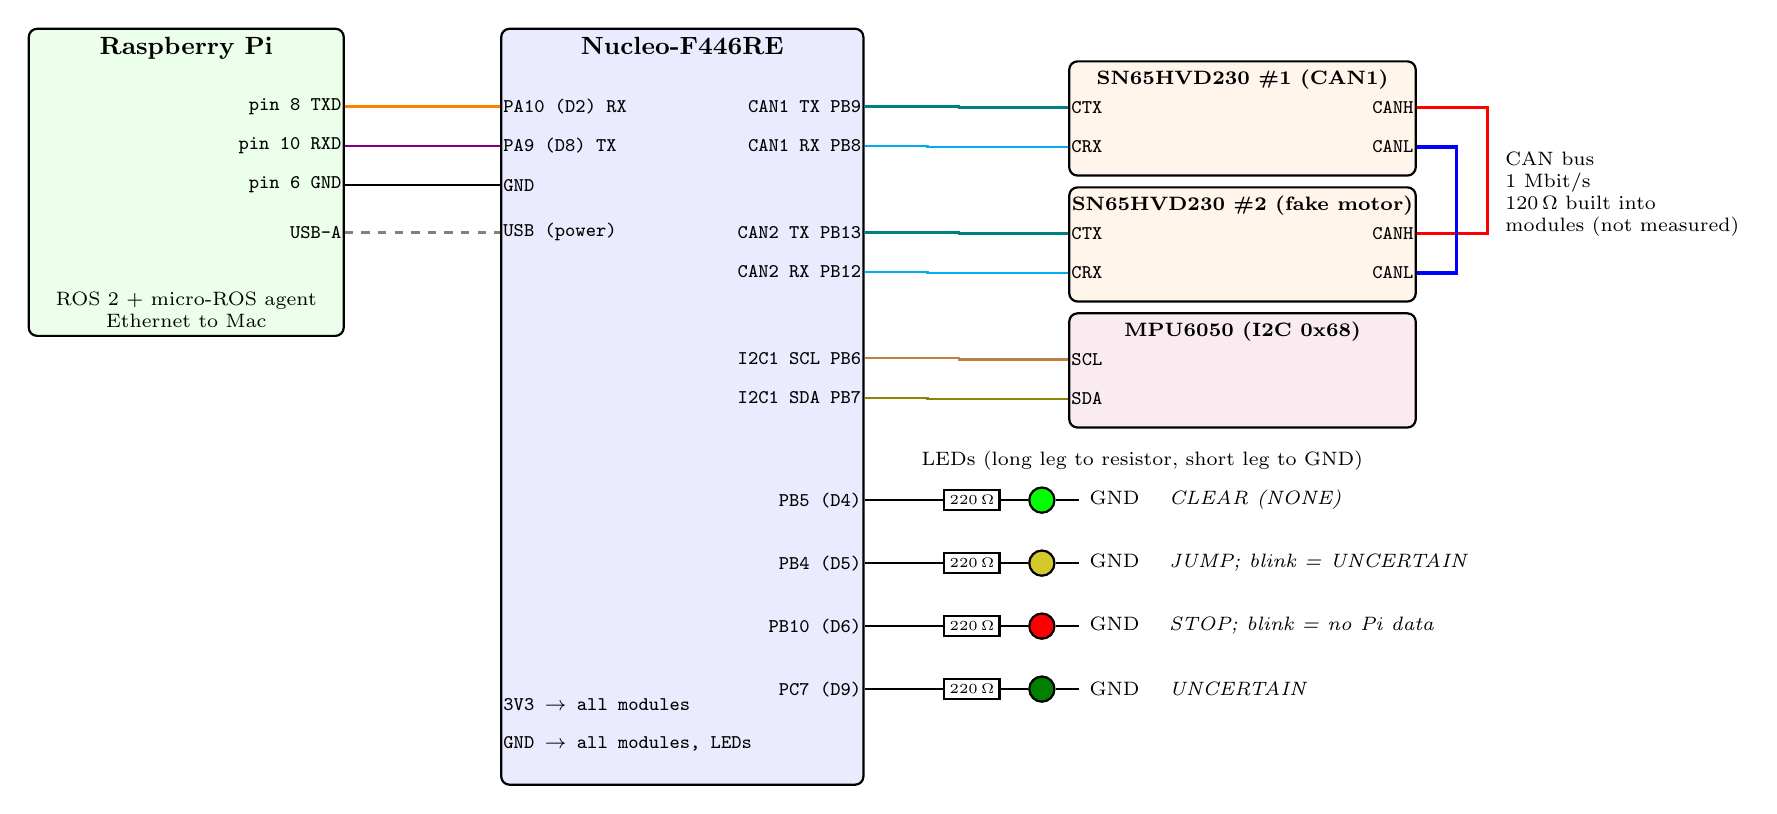
\begin{tikzpicture}
% ---------- Pi
\node[box=green,minimum height=3.9cm,minimum width=4cm] (pi) at (0,-1.35) {};
\node[font=\bfseries\small,anchor=north] at (pi.north) {Raspberry Pi};
\def\boxname{pi}
\pinrow{pi8}{1}{1.0}{pin 8 TXD}
\pinrow{pi10}{1}{1.5}{pin 10 RXD}
\pinrow{pi6}{1}{2.0}{pin 6 GND}
\pinrow{piusb}{1}{2.6}{USB-A}
\node[font=\scriptsize,anchor=south,align=center] at (pi.south) {ROS 2 + micro-ROS agent\\Ethernet to Mac};
% ---------- Nucleo
\node[box=blue,minimum height=9.6cm,minimum width=4.6cm] (nu) at (6.3,-4.2) {};
\node[font=\bfseries\small,anchor=north] at (nu.north) {Nucleo-F446RE};
\def\boxname{nu}
\pinrow{nPA10}{0}{1.0}{PA10 (D2) RX}
\pinrow{nPA9}{0}{1.5}{PA9 (D8) TX}
\pinrow{nGNDl}{0}{2.0}{GND}
\pinrow{nUSB}{0}{2.6}{USB (power)}
\pinrow{nPB9}{1}{1.0}{CAN1 TX PB9}
\pinrow{nPB8}{1}{1.5}{CAN1 RX PB8}
\pinrow{nPB13}{1}{2.6}{CAN2 TX PB13}
\pinrow{nPB12}{1}{3.1}{CAN2 RX PB12}
\pinrow{nPB6}{1}{4.2}{I2C1 SCL PB6}
\pinrow{nPB7}{1}{4.7}{I2C1 SDA PB7}
\pinrow{nPB5}{1}{6.0}{PB5 (D4)}
\pinrow{nPB4}{1}{6.8}{PB4 (D5)}
\pinrow{nPB10}{1}{7.6}{PB10 (D6)}
\pinrow{nPC7}{1}{8.4}{PC7 (D9)}
\pinrow{n33}{0}{8.6}{3V3 $\rightarrow$ all modules}
\pinrow{nGND}{0}{9.1}{GND $\rightarrow$ all modules, LEDs}
% Pi-Nucleo
\draw[w=orange] (pi8) -- ++(1.2,0) |- (nPA10);
\draw[w=violet] (pi10) -- ++(0.8,0) |- (nPA9);
\draw[w=black] (pi6) -- ++(0.4,0) |- (nGNDl);
\draw[w=gray,dashed] (piusb) -- ++(0.3,0) |- (nUSB);
% ---------- CAN1
\node[box=orange,minimum height=1.45cm,minimum width=4.4cm,anchor=north west] (c1) at (11.2,0.2) {};
\node[font=\bfseries\scriptsize,anchor=north] at (c1.north) {SN65HVD230 \#1 (CAN1)};
\def\boxname{c1}
\pinrow{c1tx}{0}{0.6}{CTX}
\pinrow{c1rx}{0}{1.1}{CRX}
\pinrow{c1h}{1}{0.6}{CANH}
\pinrow{c1l}{1}{1.1}{CANL}
\draw[w=teal] (nPB9) -- ($(nPB9)+(1.2,0)$) |- (c1tx);
\draw[w=cyan] (nPB8) -- ($(nPB8)+(0.8,0)$) |- (c1rx);
% ---------- CAN2
\node[box=orange,minimum height=1.45cm,minimum width=4.4cm,anchor=north west] (c2) at (11.2,-1.4) {};
\node[font=\bfseries\scriptsize,anchor=north] at (c2.north) {SN65HVD230 \#2 (fake motor)};
\def\boxname{c2}
\pinrow{c2tx}{0}{0.6}{CTX}
\pinrow{c2rx}{0}{1.1}{CRX}
\pinrow{c2h}{1}{0.6}{CANH}
\pinrow{c2l}{1}{1.1}{CANL}
\draw[w=teal] (nPB13) -- ($(nPB13)+(1.2,0)$) |- (c2tx);
\draw[w=cyan] (nPB12) -- ($(nPB12)+(0.8,0)$) |- (c2rx);
% CAN bus
\draw[w=red,very thick] (c1h) -- ++(0.9,0) |- (c2h);
\draw[w=blue,very thick] (c1l) -- ++(0.5,0) |- (c2l);
\node[font=\scriptsize,align=left,anchor=west] at ($(c1h)+(1.0,-1.1)$) {CAN bus\\1 Mbit/s\\120\,$\Omega$ built into\\modules (not measured)};
% ---------- MPU6050
\node[box=purple,minimum height=1.45cm,minimum width=4.4cm,anchor=north west] (imu) at (11.2,-3.0) {};
\node[font=\bfseries\scriptsize,anchor=north] at (imu.north) {MPU6050 (I2C 0x68)};
\def\boxname{imu}
\pinrow{iscl}{0}{0.6}{SCL}
\pinrow{isda}{0}{1.1}{SDA}
\draw[w=brown] (nPB6) -- ($(nPB6)+(1.2,0)$) |- (iscl);
\draw[w=olive] (nPB7) -- ($(nPB7)+(0.8,0)$) |- (isda);
% ---------- LEDs
\foreach \p/\c/\t [count=\i] in {nPB5/green/CLEAR (NONE),nPB4/yellow!80!black/JUMP; blink = UNCERTAIN,nPB10/red/STOP; blink = no Pi data,nPC7/green!50!black/UNCERTAIN / stale} {
  \draw[thick] (\p) -- ++(1.0,0) node[draw,fill=white,minimum width=0.7cm,minimum height=0.25cm,inner sep=0pt,anchor=west,font=\tiny] (r\i) {220\,$\Omega$};
  \draw[thick] (r\i.east) -- ++(0.35,0) node[circle,draw,fill=\c,minimum size=0.32cm,inner sep=0pt,anchor=west] (l\i) {};
  \draw[thick] (l\i.east) -- ++(0.3,0) node[anchor=west,font=\scriptsize] {GND \quad \textit{\t}};
}
\node[font=\scriptsize,anchor=north west] at ($(nPB5)+(0.6,0.75)$) {LEDs (long leg to resistor, short leg to GND)};
\end{tikzpicture}
\end{document}
